\documentclass{article}

\title{EE 371 Autumn 2016 - Lab 1}
\date{\today}
\author{William Li, Jun Park, Dawn Liang}

\usepackage{listings}
\usepackage{color}
\usepackage{graphicx}
\usepackage{titlesec}

\usepackage[margin=1in]{geometry}
\usepackage[document]{ragged2e}

\titleformat{\section}{\Large\bfseries}{\thesection}{0.5em}{\uppercase}

\definecolor{dkgreen}{rgb}{0,0.6,0}
\definecolor{gray}{rgb}{0.5,0.5,0.5}
\definecolor{mauve}{rgb}{0.58,0,0.82}

\lstset{frame=tb,
  language=Verilog,
  aboveskip=3mm,
  belowskip=3mm,
  showstringspaces=false,
  columns=flexible,
  basicstyle={\small\ttfamily},
  numbers=none,
  numberstyle=\tiny\color{gray},
  keywordstyle=\color{blue},
  commentstyle=\color{dkgreen},
  stringstyle=\color{mauve},
  breaklines=true,
  breakatwhitespace=true,
  tabsize=3
}

\begin{document}

\maketitle
\newpage

\tableofcontents
\newpage

\pagenumbering{arabic}

\section{Abstract}
\paragraph{} This lab focuses on introducing us to the tools and methods of digital design. We were introduced to the various levels of abstraction in modeling and implementation, the tools involved in designing and testing hardware applications, as well as the overall design process for hardware and software and applications.

\section{Introduction}
\paragraph{} First, we built four different types of counters using different modeling techniques: a 4-bit ripple up counter using gate modeling, a 4-bit synchronous up counter using both dataflow model and schematic entry, and a 4-bit synchronous Johnson up counter using the behavioural model. In the process of building and testing these counters, we were introduced to Icarus Verilog (iVerilog) and GTKWave software, for compiling our designs and simulating waveforms. We then loaded our designs onto an Altera Cyclone V FPGA, where we verified their functionality on hardware. Then we utilised Signal Tap II, a logic analyzer for probing designs in hardware. Finally, we were briefly introduced to the C programming language. We learned the basics of a C program in the CodeBlocks IDE by compiling a provided C project, and then we built a simple C car price calculator program that asks for relevant input data and outputs an approximate list price for a brand new vehicle.

\section{Discussion}
  \subsection{Design}

  \paragraph{Design Specification} We built four 4-bit counters: a ripple-up counter, two synchronous up counters, and a Johnson counter. Each counter had an active-low reset. 

  Additionally, we built a car list price calculator. Given the appropriate input data, the calculator would compute the estimated list price of a brand new vehicle.

  \paragraph{Design Procedure} In Verilog HDL, we designed and implemented four counters using the four different levels of modeling. The first three counters were implemented using the D-flipflop provided in the lab spec; the fourth counter was implemented via Quartus' schematic entry feature.

  \lstinputlisting[language=Verilog]{../counters/DFlipFlop.v}

  \paragraph{}The ripple-up counter was implemented at the structural level. The connections between the D-flipflops were explicitly assigned based on the gate level diagram.

  \paragraph{}The first synchronous up counter was implemented at the data flow level. We diagrammed the states and generated boolean expressions using truth tables and K-maps.

  \paragraph{}The johnson counter was implemented at the behavioural level. 

  \paragraph{}The second synchronous up counter was built via schematic entry.

  In this subsection you will first describe how you developed your the hardware and software for your design. You might want to include Verilog or C code fragments to illustrate specific points, the theorems you used to simplify logic expressions, the K-map(s) or the truth tables you used to simplify or verify your conclusion if that these are tools you used. 

  \paragraph{System Description} The four counters take a clock and reset as the input, and output 4-bits counting up in binary. The fourth counter also takes an enable input, determining whether the counter is on/off.

  \paragraph{} The list price calculator takes the manufacturer's cost (\$), the estimated markup (\%), the pre-tax discount (\%), and sales tax (\%) as inputs. It outputs the estimated list price of a vehicle, calculated from those values.
  
  \paragraph{Software Implementation} 

  What is your design????

Present your design starting from a top level functional view and potentially block diagram or high level architecture.  Refine that view to present and explain each of the modules that comprise the major functional blocks.  Discuss the flow of control through the design.  Identify and discuss the specific processes/tasks you have implemented in your design. Explain your design choices. 

  \paragraph{Hardware Implementation}

  See software implementation.  Now, draw the block diagrams of how you connected interconnected the major / minor modules in your system.

Include your logic equations and diagrams as well.

  \subsection{Test}

  \paragraph{Test plan}

  \paragraph{Test Specification}

  \paragraph{Test Cases}

\section{Results}

\section{Analysis of errors}

\section{Summary and Conclusion}

\section{Appendix}

\subsection{Designing and building VHDL applications - counters}

\subsubsection{Ripple up counter}
\lstinputlisting[language=Verilog]{../counters/rippleUpCounter.v}
\lstinputlisting[language=Verilog]{../counters/rippleUpCounter_tester.v}
\newpage

\begin{figure}
  \centering
	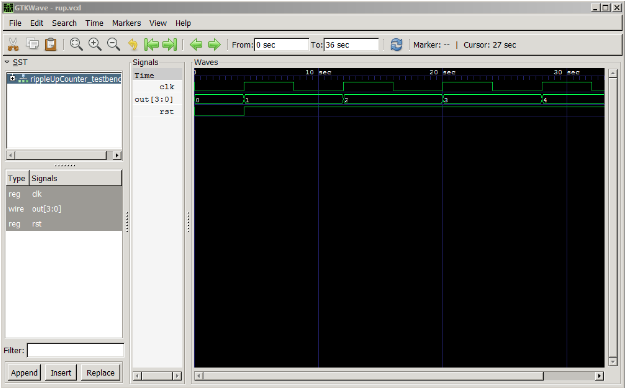
\includegraphics[width=\linewidth]{figures/waveforms/rippleUp_wave.png}
	\caption{Ripple-up counter waveform in gtkwave}
	\label{fig:rippleUp_waveform}

	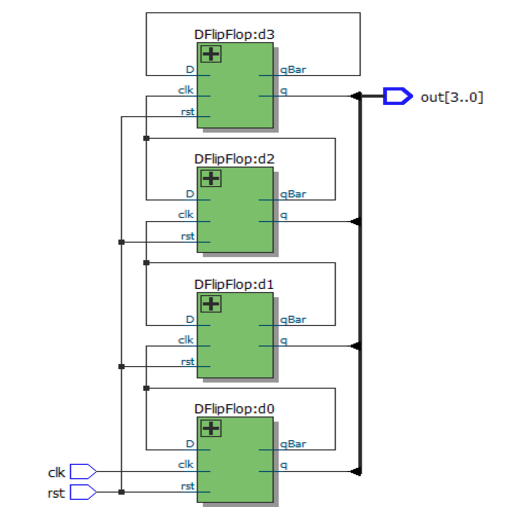
\includegraphics[width=0.75\linewidth]{figures/RTLs/rippleUp_RTL.png}
	\caption{Ripple-up counter RTL view}
	\label{fig:rippleUp_RTL}
\end{figure}
\newpage

\subsubsection{Synchronous up counter}
\lstinputlisting[language=Verilog]{../counters/synUpCounter.v}
\lstinputlisting[language=Verilog]{../counters/synUpCounter_tester.v}
\newpage

\begin{figure}
  \centering
  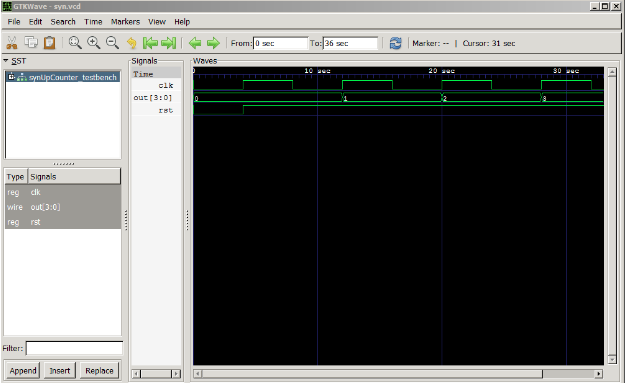
\includegraphics[width=\linewidth]{figures/waveforms/synUp_wave.png}
  \caption{Ripple-up counter waveform in gtkwave}
  \label{fig:synUp_waveform}

  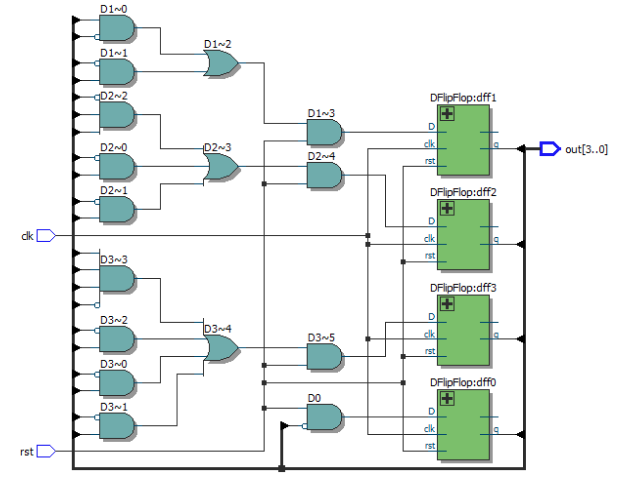
\includegraphics[width=0.75\linewidth]{figures/RTLs/synUp_RTL.png}
  \caption{Ripple-up counter RTL view}
  \label{fig:synUp_RTL}
\end{figure}
\newpage

\subsubsection{Johnson up counter}
\lstinputlisting[language=Verilog]{../counters/johnsonUpCounter.v}
\lstinputlisting[language=Verilog]{../counters/johnsonUpCounter_tester.v}
\newpage

\begin{figure}
  \centering
  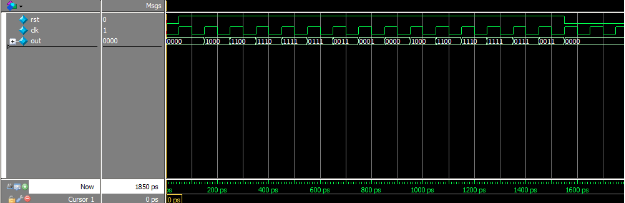
\includegraphics[width=\linewidth]{figures/waveforms/johnson_wave.png}
  \caption{Ripple-up counter waveform in gtkwave}
  \label{fig:johnson_waveform}

  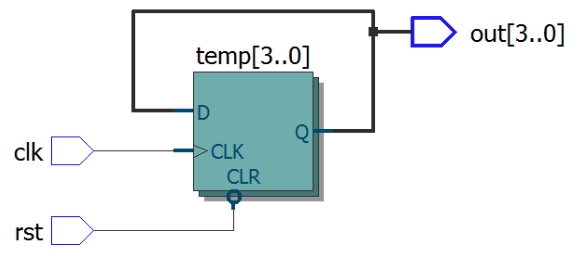
\includegraphics[width=0.75\linewidth]{figures/RTLs/johnson_RTL.png}
  \caption{Ripple-up counter RTL view}
  \label{fig:johnson_RTL}
\end{figure}
\newpage

\subsubsection{Synchronous up counter (schematic entry)}
\newpage

\begin{figure}
  \centering
  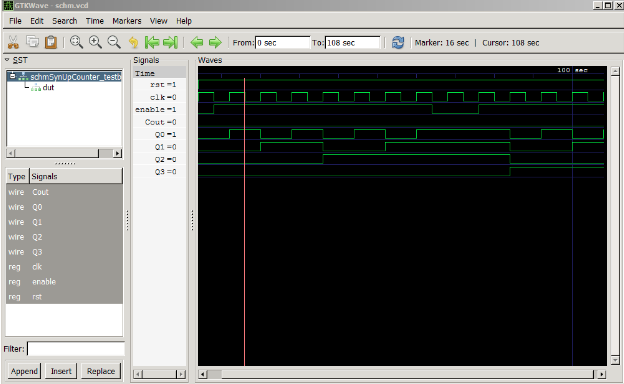
\includegraphics[width=\linewidth]{figures/waveforms/schem_synUp_wave.png}
  \caption{Ripple-up counter waveform in gtkwave}
  \label{fig:schem_synUp_waveform}

  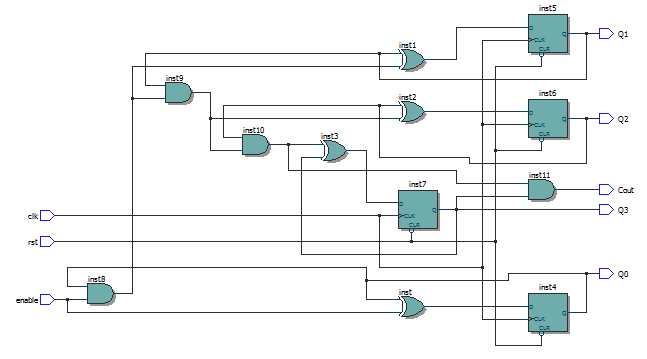
\includegraphics[width=0.75\linewidth]{figures/RTLs/schem_synUp_RTL.png}
  \caption{Ripple-up counter RTL view}
  \label{fig:schem_synUp_RTL}
\end{figure}
\newpage

\subsection{Learning the C language}

\lstinputlisting[language=C]{../listPrice/listPrice/main.c}

\section{Failure Modes Analysis}

\end{document}